%\documentclass[a4paper,superscriptaddress,11pt]{quantumarticle}
%\documentclass[aps,twocolumn,longbibliography,english,superscriptaddress]{revtex4-1}
\documentclass{article}
\usepackage{iclr2021_conference}
%\documentclass[a4paper,superscriptaddress,11pt]{article}
\pdfoutput=1
\usepackage[colorlinks=true,urlcolor=blue,citecolor=blue,linkcolor=blue]{hyperref}
\usepackage[english]{babel}
\usepackage[utf8]{inputenc}
\usepackage[T1]{fontenc}
\usepackage{amssymb}
\usepackage{tabularx}
\usepackage{quoting}
\usepackage{upquote}
\usepackage{subcaption}
\usepackage{multicol}
\usepackage[framemethod=TikZ]{mdframed}
\usepackage{wrapfig}
%\usepackage{caption}
%\usepackage[plain]{algorithm}
\usepackage[ruled, vlined]{algorithm2e}
\usepackage{algpseudocode}
\usepackage{rotating}
%\usepackage{cite}
\usepackage{booktabs}
%\usepackage{unicode-math}
%\usepackage{algorithm}% http://ctan.org/pkg/algorithm
%\usepackage{algpseudocode}% http://ctan.org/pkg/algpseudocode
\usepackage{xcolor}% http://ctan.org/pkg/xcolor
\makeatletter
\newsavebox{\@brx}
\newcommand{\llangle}[1][]{\savebox{\@brx}{\(\m@th{#1\langle}\)}%
  \mathopen{\copy\@brx\kern-0.5\wd\@brx\usebox{\@brx}}}
\newcommand{\rrangle}[1][]{\savebox{\@brx}{\(\m@th{#1\rangle}\)}%
  \mathclose{\copy\@brx\kern-0.5\wd\@brx\usebox{\@brx}}}
\makeatother
\usepackage{bbm}
\usepackage{jlcode}
\usepackage{graphicx}
\usepackage{amsmath,color,amsthm}
\usepackage{mathrsfs}
\usepackage{float}
\usepackage[normalem]{ulem}
\usepackage{makecell}
\usepackage{indentfirst}
\usepackage{txfonts}
\usepackage[epsilon, tsrm, altpo]{backnaur}

\newcommand{\listingcaption}[1]%
{%
\refstepcounter{lstlisting}\hfill%
Listing \thelstlisting: #1\hfill%\hfill%
}%
\newcolumntype{b}{X}
\newcolumntype{s}{>{\hsize=.7\hsize}X}
\usepackage{listings}
\lstset{
    language=Julia,
    basicstyle=\ttfamily\scriptsize,
    numberstyle=\scriptsize,
    % numbers=left,
    backgroundcolor=\color{gray!7},
    %backgroundcolor=\color{white},
    %frame=single,
    xleftmargin=2em,
    tabsize=2,
    rulecolor=\color{black!15},
    %title=\lstname,
    escapeinside={(*}{*)},
    breaklines=true,
    %breakatwhitespace=true,
    %framextopmargin=2pt,
    %framexbottommargin=2pt,
    frame=bt,
    extendedchars=true,
    inputencoding=utf8,
    columns=fullflexible,
    %escapeinside={(*@}{@*)},
}

\tolerance=1
\emergencystretch=\maxdimen
\hyphenpenalty=1000
\hbadness=1000

\makeatletter

%%%%%%%%%%%%%%%%%%%%%%%%%%%%%% User specified LaTeX commands.

%Journal reference.  Comma sets off: name, vol, page, year
\def\journal #1, #2, #3, 1#4#5#6{{\sl #1~}{\bf #2}, #3 (1#4#5#6) }
\def\pr{\journal Phys. Rev., }
\def\prb{\journal Phys. Rev. B, }
\def\prl{\journal Phys. Rev. Lett., }
\def\pl{\journal Phys. Lett., }
%\def\np{\journal Nucl. Phys., }


%%%%%%%%%%%%%%%%%%%%%%%%%%%%%%%%%%%%%%%%%%%%%%%%%%%%%%%%%%%%%%%%%%%%%%%%%%%%%%%%%%%%%%%%%%%%%%%%%%%%%%%%%%%%%%%%%%%%%%%%%%%%%%%%%%%%%%%%%%%%%%%%%%%%%%%%%%%%%%%%%%%%%%%%%%%%%%%%%%%%%%%%%%%%%%%%%%%%%%%%%%%%%%%%%%%%%%%%%%%%%%%%%%%%%%%%%%%%%%%%%%%%%%%%%%%%


%\usepackage{CJK}
%\usepackage[colorlinks, citecolor=blue]{hyperref}
\DeclareMathOperator*{\argmax}{arg\,max}

%%%%%% Shortcut related
\newcommand{\<}{\langle}
\renewcommand{\>}{\rangle}
\newcommand{\out}{{\vx^L}}
\newcommand{\inp}{{\vx^0}}
\newcommand{\cquad}{{{ }_{\quad}}}
\newcommand{\pluseq}{\mathrel{+}=}
\newcommand{\minuseq}{\mathrel{-}=}
\newcommand{\vx}{{\mathbf{x}}}
\newcommand{\vg}{{\mathbf{g}}}
\newcommand{\vp}{{\mathbf{p}}}
\newcommand{\vy}{{\mathbf{y}}}
\newcommand{\Var}{{\mathrm{Var}}}
\newcommand{\Mean}{{\mathrm{E}}}
\newcommand{\vvalue}{{\texttt{value}}}
\newcommand{\grad}{{\texttt{grad}}}
\newcommand{\parameter}{{\texttt{parameter}}}
%%%%%% Convention related
\newcommand{\SWAP}{{\rm SWAP}}
\newcommand{\CNOT}{{\rm CNOT}}
\newcommand{\bigO}{{\mathcal{O}}}
\newcommand{\X}{{\rm X}}
\renewcommand{\H}{{\rm H}}
\newcommand{\Rx}{{\rm Rx}}
\renewcommand{\v}[1]{{\bf #1}}
\newcommand{\dataset}{{\mathcal{D}}}
\newcommand{\wfunc}{{\psi}}
\newcommand{\SU}{{\rm SU}}
\newcommand{\UU}{{\rm U}}
\newcommand{\thetav}{{\boldsymbol{\theta}}}
\newcommand{\gammav}{{\boldsymbol{\gamma}}}
\newcommand{\thetai}{{\theta^\alpha_l}}
\newcommand{\Expect}{{\mathbb{E}}}
\newcommand{\Tr}{{\rm Tr}}
\renewcommand{\cite}[1]{{\citep{#1}}}
\newcommand{\etc}{{\it etc~}}
\newcommand{\etal}{{\it etal~}}
\newcommand{\xset}{\mathbf{X}}
\newcommand{\fl}{\texttt{fl}}
\newcommand{\pdata}{\mathbf{\pi}}
\newcommand{\q}{\mathbf{q}}
\newcommand{\epdata}{\mathbf{\hat{\pi}}}
\newcommand{\gammaset}{\boldsymbol{\Gamma}}
\newcommand{\ei}{{\mathbf{e}_l^\alpha}}
\newcommand{\vtheta}{{\boldsymbol{\theta}}}
\newcommand{\sigmag}{{\nu}}
\newcommand{\sigmai}[2]{{\sigma^{#2}_{#1}}}
\newcommand{\qi}[1]{{q^{\alpha_{#1}}_{#1}}}
\newcommand{\BAS}{Bars-and-Stripes}
\newcommand{\circled}[1]{\raisebox{.5pt}{\textcircled{\raisebox{-.9pt} {#1}}}}
\newcommand{\qexpect}[1]{{\left\langle #1\right\rangle}}
\newcommand{\expect}[2]{{\mathop{\mathbb{E}}\limits_{\substack{#2}}\left[#1\right]}}
\newcommand{\var}[2]{{\mathop{\mathrm{Var}}\limits_{\substack{#2}}\left(#1\right)}}
\newcommand{\pshift}[1]{{p_{\thetav+#1}}}
\newcommand{\upcite}[1]{\textsuperscript{\cite{#1}}}
\newcommand{\Eq}[1]{Eq.~(\ref{#1})}
\newcommand{\Fig}[1]{Fig.~\ref{#1}}
\newcommand{\Lst}[1]{Listing.~\ref{#1}}
\newcommand{\Tbl}[1]{Table~\ref{#1}}
\newcommand{\Sec}[1]{Sec.~\ref{#1}}
\newcommand{\App}[1]{Appendix~\ref{#1}}
\newcommand{\bra}[1]{\mbox{$\left\langle #1 \right|$}}
\newcommand{\ket}[1]{\mbox{$\left| #1 \right\rangle$}}
\newcommand{\braket}[2]{\mbox{$\left\langle #1 | #2 \right\rangle$}}
\newcommand{\tr}[1]{\mathrm{tr}\mbox{$\left[ #1\right]$}}

\newcommand{\ra}[1]{\renewcommand{\arraystretch}{#1}}

%%%%%% Comment related
\newcommand{\red}[1]{[{\bf  \color{red}{LW: #1}}]}
\newcommand{\xred}[1]{[{\bf  \color{red}{\sout{LW: #1}}}]}
\newcommand{\blue}[1]{[{\bf  \color{blue}{JG: #1}}]}
\newcommand{\violet}[1]{[{\bf  \color{violet}{MLS: #1}}]}
\newcommand{\green}[1]{[{\bf  \color{green}{TZ: #1}}]}
\newcommand{\xgreen}[1]{[{\bf  \color{green}{\sout{TZ: #1}}}]}
\newcommand{\xblue}[1]{[{\bf  \color{blue}{\sout{JG: #1}}}]}
\newcommand{\material}[1]{\iffalse[{\bf  \color{cyan}{Material: #1}}]\fi}
\newcommand{\orange}[1]{\iffalse[{\bf  \color{orange}{Jo: #1}}]\fi}

\newtheorem{theorem}{\textit{Rule}}
\theoremstyle{definition}\newtheorem{definition}{\textit{Definition}}

\makeatother

\iclrfinalcopy
\begin{document}
\title{Solving the maximum independant set problem with tensor networks}

\author{Jin-Guo Liu\\
Harvard University\\
\texttt{jinguoliu@g.harvard.edu}\\
\AND
Xun Gao\\
Harvard University\\
\texttt{xungao@g.harvard.edu}\\
%\AND
%Sheng-Tao Wang\\
%QuEra computing Inc.
}
\maketitle

\begin{abstract}
	Solving the maximum independent set size problem: the maximum independent set size, the independance polynomial and the optimal configuration.
\end{abstract}

\section{Technical guide}
\begin{description}
	\item[OMEinsum] a package for einsum,
	\item[OMEinsumContractionOrders] a package for finding the optimal contraction order for einsum \\ \href{https://github.com/Happy-Diode/OMEinsumContractionOrders.jl}{https://github.com/Happy-Diode/OMEinsumContractionOrders.jl},
	\item[TropicalGEMM] a package for efficient tropical matrix multiplication (compatible with OMEinsum),
	\item[TropicalNumbers] a package providing tropical number types and tropical algebra, one o the dependency of TropicalGEMM,
	\item[LightGraphs] a package providing graph utilities, like random regular graph generator,
	\item[Polynomials] a package providing polynomial algebra and polynomial fitting,
	\item[Mods and Primes] packages providing finite field algebra and prime number generators.
\end{description}

One can install these packages by opening a julia REPL, type \colorbox{lightgray}{\texttt{]}} to enter the \texttt{pkg>} mode and type, e.g.
\begin{lstlisting}
pkg> add OMEinsum
\end{lstlisting}

An example of computing the maximum independant set size
\begin{lstlisting}
julia> using OMEinsum, LightGraphs, TropicalNumbers

julia> n, k = 6, 3
(6, 3)

julia> g = LightGraphs.random_regular_graph(n, k)
{6, 9} undirected simple Int64 graph

julia> ixs = [minmax(e.src,e.dst) for e in LightGraphs.edges(g)]
9-element Vector{Tuple{Int64, Int64}}:
 (1, 2)
 (1, 4)
 (1, 5)
 (2, 3)
 (2, 6)
 (3, 5)
 (3, 6)
 (4, 5)
 (4, 6)

julia> code = EinCode((ixs..., [(i,) for i in LightGraphs.vertices(g)]...), ())
1∘2, 1∘4, 1∘5, 2∘3, 2∘6, 3∘5, 3∘6, 4∘5, 4∘6, 1, 2, 3, 4, 5, 6 -> 

julia> optimized_code = optimize_greedy(code, Dict([i=>2 for i=1:6]))
4∘6, 4∘6 -> 
├─ 4∘6, 6 -> 4∘6
│  ├─ 6
│  └─ 4∘6
└─ 2∘5∘4, 5∘2∘6 -> 4∘6
   ├─ 2∘5∘6, 6∘2 -> 5∘2∘6
   │  ├─ 2∘6, 2 -> 6∘2
   │  │  ├─ 2
   │  │  └─ 2∘6
   │  └─ 2∘3, 5∘6∘3 -> 2∘5∘6
   │     ├─ 3∘5, 6∘3 -> 5∘6∘3
   │     │  ├─ 3∘6, 3 -> 6∘3
   │     │  │  ⋮
   │     │  │  
   │     │  └─ 3∘5, 5 -> 3∘5
   │     │     ⋮
   │     │     
   │     └─ 2∘3
   └─ 2∘4∘1, 1∘4∘5 -> 2∘5∘4
      ├─ 1∘5, 5∘4 -> 1∘4∘5
      │  ├─ 4∘5, 4 -> 5∘4
      │  │  ├─ 4
      │  │  └─ 4∘5
      │  └─ 1∘5
      └─ 2∘1, 1∘4 -> 2∘4∘1
         ├─ 1∘4
         └─ 1∘2, 1 -> 2∘1
            ├─ 1
            └─ 1∘2


julia> function mis_contract(code::OMEinsum.NestedEinsum, x::T) where T
           tensors = map(OMEinsum.getixs(Iterators.flatten(code))) do ix
               @assert length(ix) == 1 || length(ix) == 2
                           length(ix) == 1 ? [one(T), x] : [one(T) one(T); one(T) zero(T)]
           end
                 code(tensors...)
       end
mis_contract (generic function with 1 method)

julia> result = mis_contract(optimized_code, Tropical(1.0))
0-dimensional Array{TropicalF64, 0}:
2.0ₜ
\end{lstlisting}

For larger graph, we hight recommend using two additional packages,
\texttt{TropicalGEMM} for BLAS speed tropical matrix multiplication and
\texttt{OMEinsumContractionOrders} for hyper optimized contraction order (the KaHyPar approach) ~\cite{Gray2021,Pan2021}.

\section{Computing degeneracy}
Consider the following 5 node graph.

\begin{figure}[H]
    \centerline{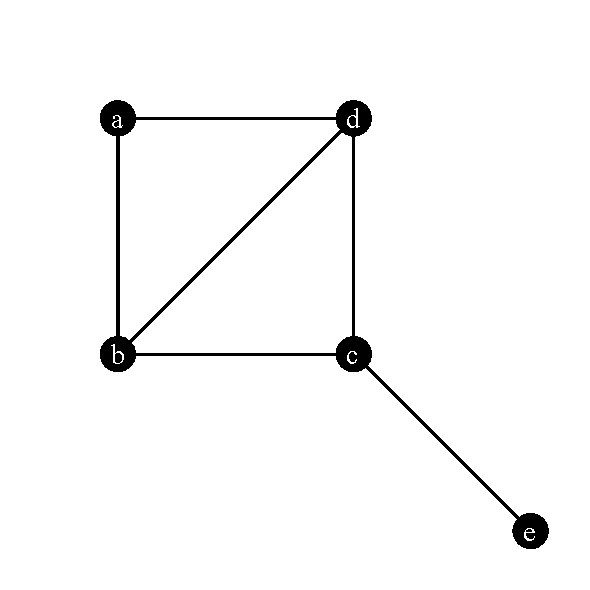
\includegraphics[width=0.4\columnwidth,trim={0 0cm 0 0},clip]{../notebooks/fig1.pdf}}
\end{figure}

If put a vector of size $2$ at each vertex
\begin{equation}
    \left(\begin{matrix}
        1 \\
        x
    \end{matrix}\right),
\end{equation}
were $x$ is a variable, and a matrix of size $2 \times 2$ at each edge
\begin{equation}
    \left(\begin{matrix}
        1  & 1\\
        1 & 0
    \end{matrix}\right).
\end{equation}

\begin{figure}[H]
    \centerline{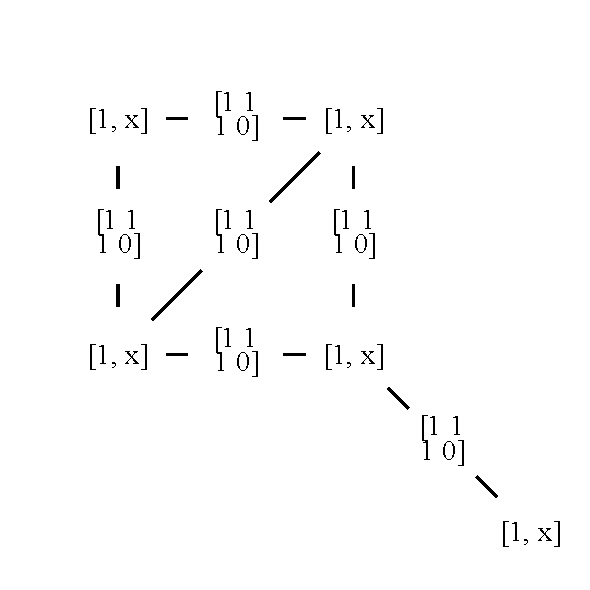
\includegraphics[width=0.4\columnwidth,trim={0 0cm 0 0},clip]{../notebooks/fig2.pdf}}
\end{figure}

Then we contract this graph with einsum \texttt{a,b,c,d,ab,ad,bc,bd,cd,ce->}.
The result is a scalar function of $x$, it corresponds to the independance polynomial~\cite{}.
\begin{equation}
I(G, x) = \sum_{k=1}^{\alpha(G)} a_k x^k,
\end{equation}
where $a_k$ is the the degeneracy for independant set size $k$.

\subsection{Symbolic computing}
The most straight forward approach is the symbolic computing, where we store a polynomial of $x$ as a vector of factors.
We define the algebra between these vectors of factors and insert them to the original tensor network contraction algorithm.
However, this method suffers from a space overhead that propotional to the maximum independant set size.

\subsection{Polynomial fitting}
Let $m$ be the maximum independent set size and $X$ be a set of $m+1$ random real numbers, e.g. $\{0, 1, 2, \ldots, m\}$.
We compute the einsum contraction for each $x \in X$ and obtain the following relations
\begin{align}
a_0 + a_1 x_1 + a_1 x_1^2 + \ldots + a_m x_1^m &= y_0\\
a_0 + a_1 x_2 + a_2 x_2^2 + \ldots + a_m x_2^m &= y_1\\
\ldots&\\
a_0 + a_1 x_m + a_2 x_m^2 + \ldots + a_m x_m^m& = y_m
\end{align}
The polynomial fitting between $X$ and $Y = \{y_0, y_1, \ldots, y_m\}$ gives us the factors.

\subsection{Fourier transformation}
\begin{align}
\left(\begin{matrix}
1 & x_1 & x_1^2 & \ldots & x_1^m \\
1 & x_2 & x_2^2 & \ldots & x_2^m \\
\vdots & \vdots & \vdots &\ddots & \vdots \\
1 & x_m & x_m^2 & \ldots & x_m^m
\end{matrix}\right)
\left(\begin{matrix}
a_0 \\ a_1 \\ \vdots \\ a_m
\end{matrix}\right)
= \left(\begin{matrix}
y_0 \\ y_1 \\ \vdots \\ y_m
\end{matrix}\right)
\end{align}

\begin{align}
\left(\begin{matrix}
1 & r\omega & r^2\omega^2 & \ldots & r^m\omega^m \\
1 & r\omega^2 & r^2\omega^4 & \ldots & r^m\omega^{2m} \\
\vdots & \vdots & \vdots &\ddots & \vdots \\
1 & r\omega^m & r^2\omega^{2m} & \ldots & r^m\omega^{m^2}
\end{matrix}\right)
\left(\begin{matrix}
a_0 \\ a_1 \\ \vdots \\ a_m
\end{matrix}\right)
= \left(\begin{matrix}
y_0 \\ y_1 \\ \vdots \\ y_m
\end{matrix}\right)
\end{align}

When $r=1$, the left side is a DFT matrix. We can obtain the factors using the relation $\vec a = {\rm FFT^{-1}}(\omega) \cdot \vec y$.
In the special case that $\omega = e^{-2\pi i/(m+1)}$, it is directly solvable with inverse fast fourier transformation algorithm in package \texttt{FFTW}.

\begin{equation}
{\rm FFT}(\omega) \cdot \vec a_r = \vec y
\end{equation}
where $(\vec a_r)_k = a_k r ^k$, by choosing diferent $r$, we can obtain better precision in low independant set size region  ($\omega<1$) and high independant set size region ($\omega>1$).

\subsection{Finite field algebra}

\section{Utilizing the sparsity}
Tensor network compression is an important tool to utilize sparsity.

We contract the tensors in a subregion $R \subseteq G$ of a graph $G$, and obtain a resulting tensor $A$ of rank $|C|$, where $C$ is the set of vertice tensors at the cut.
The maximum independant set size in this region with boundary configuration $\sigma \in \{0,1\}\otimes |C|$ is $A_{\sigma}$.
We say an entry $A_{\sigma_a}$ is ``better'' than $A_{\sigma_b}$ if
\begin{align}
(\sigma_a \land \sigma_b = \sigma_a) \land (A_{\sigma_a} \geq A_{\sigma_b}),\label{eq:compress}
\end{align}
where $\land$ is a bitwise and operations.
The first term means that whenever a bit in $\sigma_a$ has boolean value $1$, the corresponding bit in $\sigma_b$ is also $1$.
While the second term means the maximum independant set size with boundary configuration fixed to $\sigma_a$ is not less than that fixed to $\sigma_b$.
The word ``better'' means the best solution with boundary configuration $\sigma_a$ is never worse than that with $\sigma_b$.
When Eq. \ref{eq:compress} holds, It is easy to see that if $\sigma_b \cup \overline{\sigma_b}$ is one of the solutions for maximum independant sets in $G$, $\sigma_a \cup \overline{\sigma_b}$ is also a solution.


\subsection{The tensor network compression detects branching rules automatically}

\textit{max-size rule} The resulting tensor of Tropical tensor contraction stores only the local independant set size that maximizes the internal degrees on freedom.
Where the internal degree of freedom are edges that does not connect to tensors not contracted.

\textit{max-interior rule} The resulting tensor of Tropical tensor contraction stores only the local independant set size that maximizes the internal degrees on freedom.

We are going the verify the Lemmas used in branching algorithm in book~\cite{Fomin2013}.
\begin{theorem}\label{rule:one} % basic
  If a vertex $v$ is in an independent set $I$, then none of its neighbors can be in $I$.
On the other hand, if $I$ is a maximum (and thus maximal) independent set,
and thus if $v$ is not in $I$ then at least one of its neighbors is in $I$.
\end{theorem}

Contract $N[v]$, each entry of the resulting tensor of rank $|N(v)|$ corresponds to a locally maximized independant set size with fixed boundary configuration.
If the boundary configuration is a bit string of 0s, $\sigma_v$ will takes value $1$ to maximize the local independant set size.

\begin{theorem} % 2.5
Let $G=(V,E)$ be a graph, let $v$ and $w$ be adjacent vertices of $G$ such that $N[v] \subseteq N[w]$. Then
\begin{equation}
\alpha(G)=\alpha(G\backslash w).
\end{equation}
\end{theorem}

Contract $N[w]$, both $\{v, w\}$ disapear from the tensor indices because they are inner degrees of freedom.
If $w$ is one, then $N[v]$ are all zeros, the resulting tensor element can not be larger than setting $v=1$ and $w=0$.
By the maximization rule, the local tensor does not change if we remove $w$.

\begin{theorem} % 2.6
  Let $G = (V, E)$ be a graph and let $v$ be a vertex of $G$. If no maximum
independent set of $G$ contains $v$ then every maximum independent set of $G$ contains
at least two vertices of $N(v)$.
\end{theorem}

\begin{theorem} % 2.7
Let $G = (V, E)$ be a graph and $v$ a vertex of $G$. Then
\begin{equation}
\alpha(G) = \max(1 + \alpha(G \backslash N[v]), \alpha(G \backslash (M(v) \cup \{v\})).
\end{equation}
\end{theorem}

Here, $M(v)$ is the set of mirrors of $v$ in $G$.
A vertex $w \in N^2(v)$ is called a mirror of $v$ if $N(v) \backslash N(w)$ is a clique.
This rule states that if $v$ is not in $M$, there exists an MIS $I$ that $M(v)\notin I$.
otherwise, there must be one of $N(v)$ in the MIS (maximization rule).
If $w$ is in $I$, then none of $N(v) \cap N(w)$ is in $I$, then there must be one of node in the clique $N(v)\backslash N(w)$ in $I$ (maximization rule),
since clique has at most one node in the MIS, the tensor compression will eliminate this solution by moving the occuppied node to the interior.
Hence, the tensor compression rule do captures the mirror rule.

\begin{theorem} % 2.9
Let $G = (V, E)$ be a graph and $v$ be a vertex of $G$ such that $N[v]$ is a
clique. Then
\begin{equation}
\alpha(G) = 1 + \alpha(G \backslash N[v]).
\end{equation}
\end{theorem}


\begin{theorem}  %2.10
Let $G$ be a graph, let $S$ be a separator of $G$ and let $I(S)$ be the set of
all subsets of $S$ being an independent set of $G$. Then
\begin{equation}
\alpha(G) = \max_{A\in I(S)} |A| + \alpha(G \backslash (S \cup N[A])).
\end{equation}
\end{theorem}

\begin{theorem}  %2.11
Let $G = (V, E)$ be a disconnected graph and $C \subseteq V$ a connected com-
ponent of $G$. Then
\begin{equation}
\alpha(G) = \alpha(G[C]) + \alpha(G \backslash C)).
\end{equation}
\end{theorem}

\begin{align}
if |V| = 0 then
return 0
if \exists v \in V with d(v) \leq 1 then
return 1 + mis2(G \backslash N[v])
if \exists v \in V with d(v) = 2 then
(let u 1 and u 2 be the neighbors of v)
if {u 1 , u 2 } \in E then
return 1 + mis2(G \backslash N[v])
if {u 1 , u 2 } \in
/ E then
if |N 2 (v)| = 1 then
(let N 2 (v) = {w})
return max(2 + mis2(G \backslash (N 2 [v] \cup N[w])), 2 + mis2(G \backslash N 2 [v]))
if |N 2 (v)| > 1 then
return max(mis2(G \backslash N[v]), mis2(G \backslash (M(v) \cup cup))
if \exists v \in V with d(v) = 3 then
(let u 1 u 2 and u 3 be the neighbors of v)
if G[N(v)] has no edge then
if v has a mirror then
return max(1 + mis2(G \backslash N[v]), mis2(G \backslash (M(v) \cup {v}))
if v has no mirror then
return max(1 + mis2(G \backslash N[v]), 2 + mis2(G \backslash N[{u 1 , u 2 }]), 2 + mis2(G \backslash
(N[{u_1 , u_3 }] \cup \{u_2\})), 2 + mis2(G \backslash (N[{u_2 , u_3 }] \cup \{1\})))
if G[N(v)] has one or two edges then
return max(1 + mis2(G \backslash N[v]), mis2(G \backslash (M(v) \cup cup))
if G[N(v)] has three edges then
return 1 + mis2(G \backslash N[v])
if \Delta (G) \geq 6 then
choose a vertex v of maximum degree in G
return max(1 + mis2(G \backslash N[v]), mis2(G \backslash v))
if G is disconnected then
(let C \subseteq V be a component of G)
return mis2(G[C]) + mis2(G \backslash C)
if G is 4 or 5-regular then
choose any vertex v of G
return max(1 + mis2(G \backslash N[v]), mis2(G \backslash (M(v) \cup \{v\}))
if \Delta (G) = 5 and \delta (G) = 4 then
choose adjacent vertices v and w with d(v) = 5 and d(w) = 4 in G
return
\max(1 + mis2(G \backslash N[v]), 1 + mis2(G \backslash (\{v\} \cup M(v) \cup N[w])), mis2(G \backslash (M(v) \cup \{v, w\})))
\end{align}

\bibliographystyle{iclr2021_conference}
\bibliography{refs}

\appendix

\end{document}
